\chapter{Silicon Photomultiplier characterization studies}
One major focus of this thesis is the characterization of SiPMs in terms of measuring IV-curves, determining the breakdown voltage and optimal working voltage, pulse shaping and comparing responses of different array setups.
\section{Development of a SiPM-board}
\begin{figure}[b!]
	\subfloat[SiPM Printed Circuit Board (PCB)] {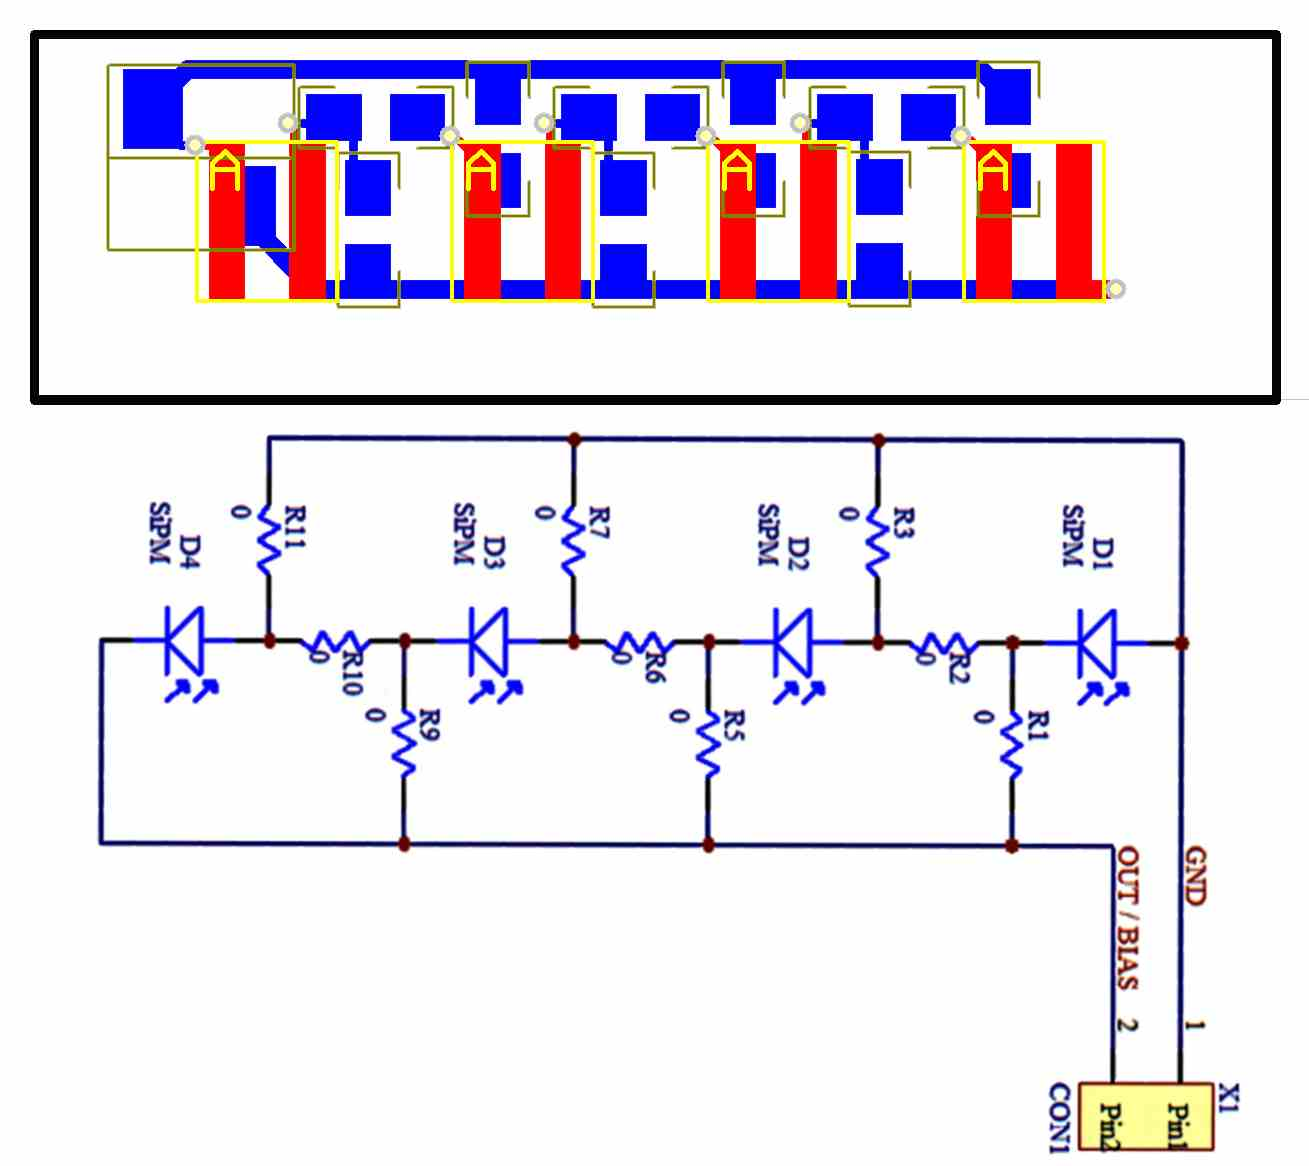
\includegraphics[width=0.49\textwidth]{./graphics/ch4/PCB.jpg}}
	\hfill
	\subfloat[SiPM circuit configurations \cite{sebastian}] {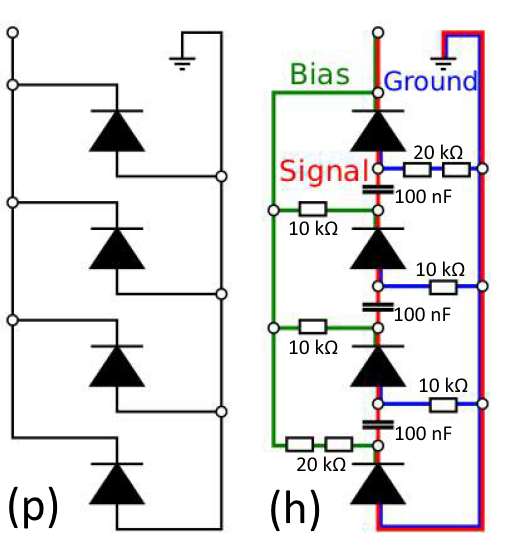
\includegraphics[width=0.4\textwidth]{./graphics/ch4/circuits.png}}
	\hfill
	\caption[SiPM circuit configurations]{SiPM board development.  }
	\label{fig:ch4:PCB}
\end{figure}
As a first approach, an electronic board for mounting different configurations of SiPMs has been developed. The PCB is shown in figure \ref{fig:ch4:PCB}. Note that this board allows different SiPM-configurations like single (s), parallel (p) and hybrid (h), the pros and cons of each will be discussed later. The design is inspired by the readout module for the scintillator tiles of the PANDA Barrel-TOF detector \cite{SciTil}. Figure \ref{fig:ch4:PCB} shows the PCB design and the circuit. A single SiPM is directly connected to the bias and ground without any passive parts. The parallel board integrates two till four SiPMs, each of them connected to the bias and ground in parallel. A fast, shaped signal is received when capacitors connect anode and cathode of adjacent SiPMs (hybrid) and resistors are used for connecting the SiPMs with bias and ground. The signal is coupled onto the DC bias voltage and can be separated via a capacitor.  \par 
For this thesis, \tit{KETEK} PM3350-EB were used. With an active area of $\SI{3}{\milli\meter}\times\SI{3}{\milli\meter}$ and a pixel size of $\SI{50}{\micro\meter}\times\SI{50}{\micro\meter}$ and 3472 pixels overall, the SiPM trades off a high photo detection efficiency and a good micro cell density. For further parameters, see \cite{SiPM_Manual}. \par
With a breakdown voltage of $U_{BD}=\SI{25}{\volt}$ and an operation voltage of $U_{OP}=U_{BD}+(2-7)\si{\volt}$, the (s)-configuration can be chosen for low cost and a fair light exposure, i.e. a plastic scintillator for measuring cosmic muons. The (h)-configuration promises good timing with a fast rising edge. It is meant for precise timing purposes, like time of flight measurements. An energy measurement can be done with the (p)-configuration, where the effective light-sensitive area is directly given by the sum of the SiPM surfaces. For some experiments, preamplifiers by \tit{Photonique} have been used \cite{photonique}.\par 

\section{Current$-$voltage characteristic}
\begin{figure}[b]
	\centering
	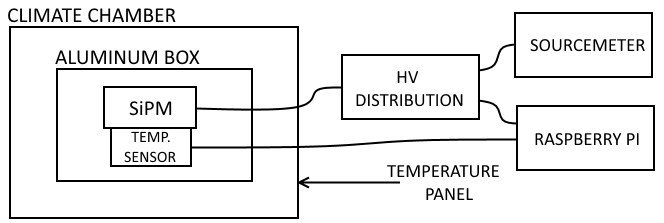
\includegraphics[width=0.85\linewidth]{./graphics/ch4/scheme_iv_curves.png}
	\caption{Schematic of the IV-characterization measurement setup.}
	\label{fig:ch4:iv_scheme}
\end{figure}
To determine the temperature dependence of the breakdown and optimal operation voltage, some IV-curve of arbitrarily chosen SiPMs in different configurations have been measured.  \par 
This setup is shown in figure \ref{fig:ch4:iv_scheme}: The climate chamber contains an aluminum box with the SiPM. The HV board \cite{chris}, which is currently under development for the EMC barrel of the PANDA experiment at FAIR (GSI) \cite{panda_emctdr}, has been chosen to perform the IV-scanning because of availability and easy programmability. The board is controlled by a Raspberry Pi 2 micro-computer which also reads out a temperature sensor  directly attached to the SiPM. To avoid parasitic light and surface leakage, the SiPM is cleaned with ethanol and is wrapped in black tape. A Keithley sourcemeter powers the HV board, a PC controls the Raspberry via Ethernet. The temperature settings can be set by a terminal. 
\begin{figure}[h!]
	\subfloat[(s)-configuration] {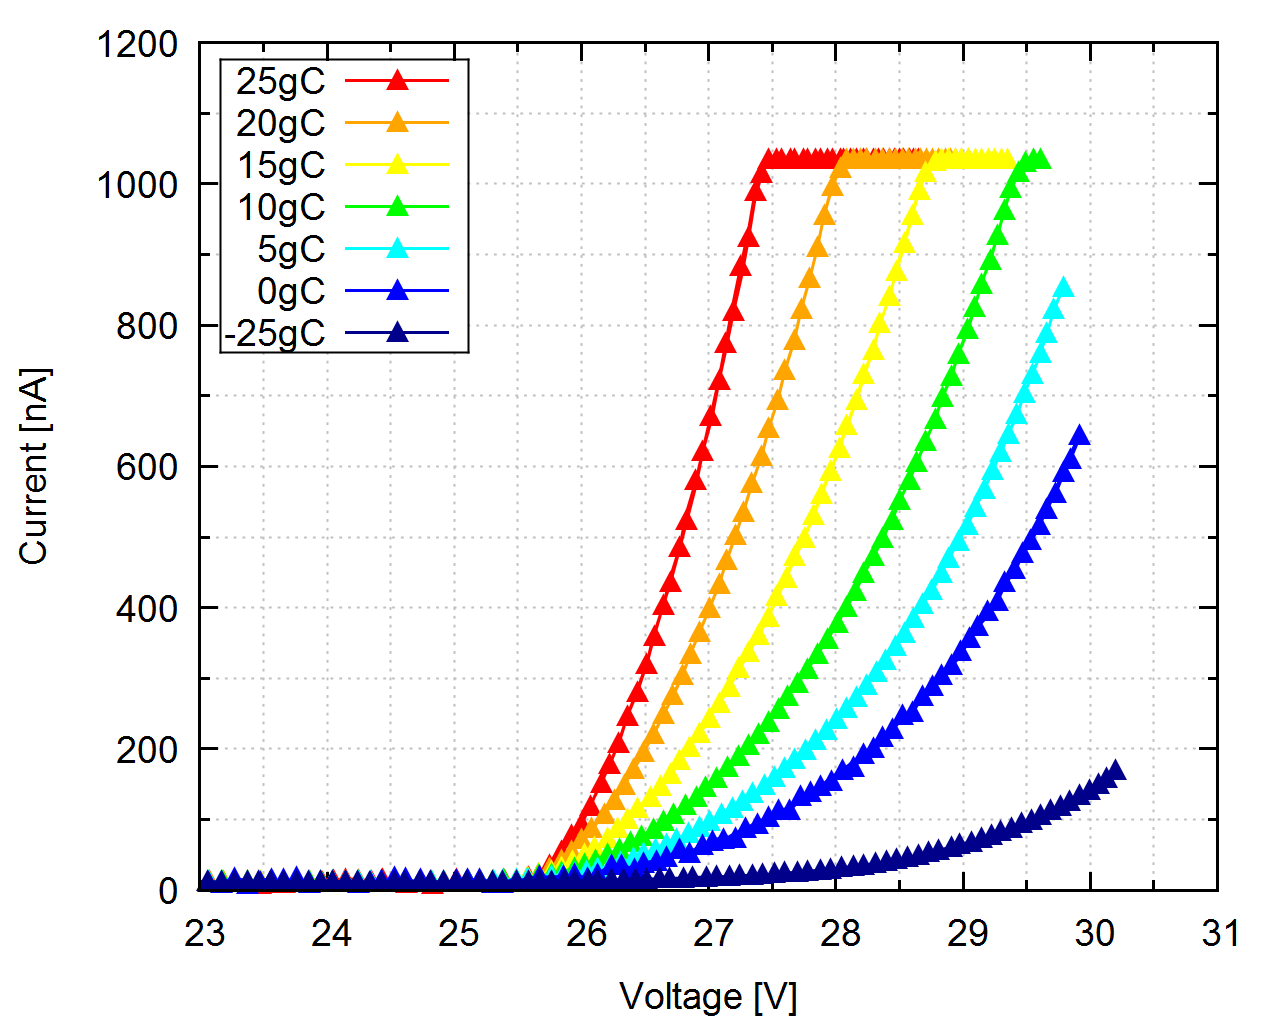
\includegraphics[width=0.49\textwidth]{./plots/iu_curve/1x1n2.png}}
	\hfill
	\subfloat[(s)-configuration logscale] {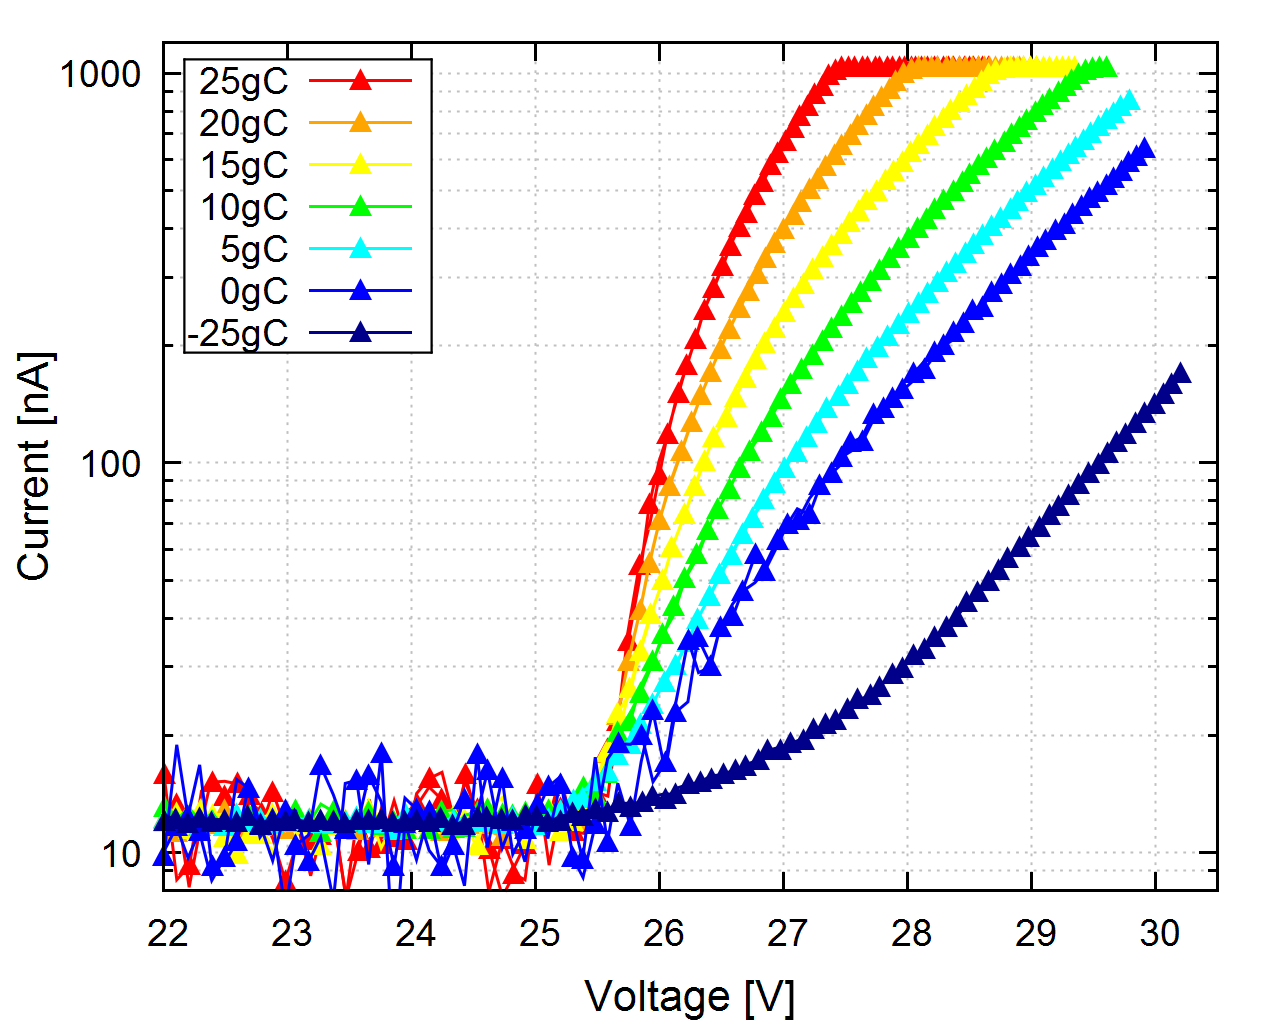
\includegraphics[width=0.49\textwidth]{./plots/iu_curve/1x1n2_log.png}}
	\hfill
	\subfloat[(h)-configuration] {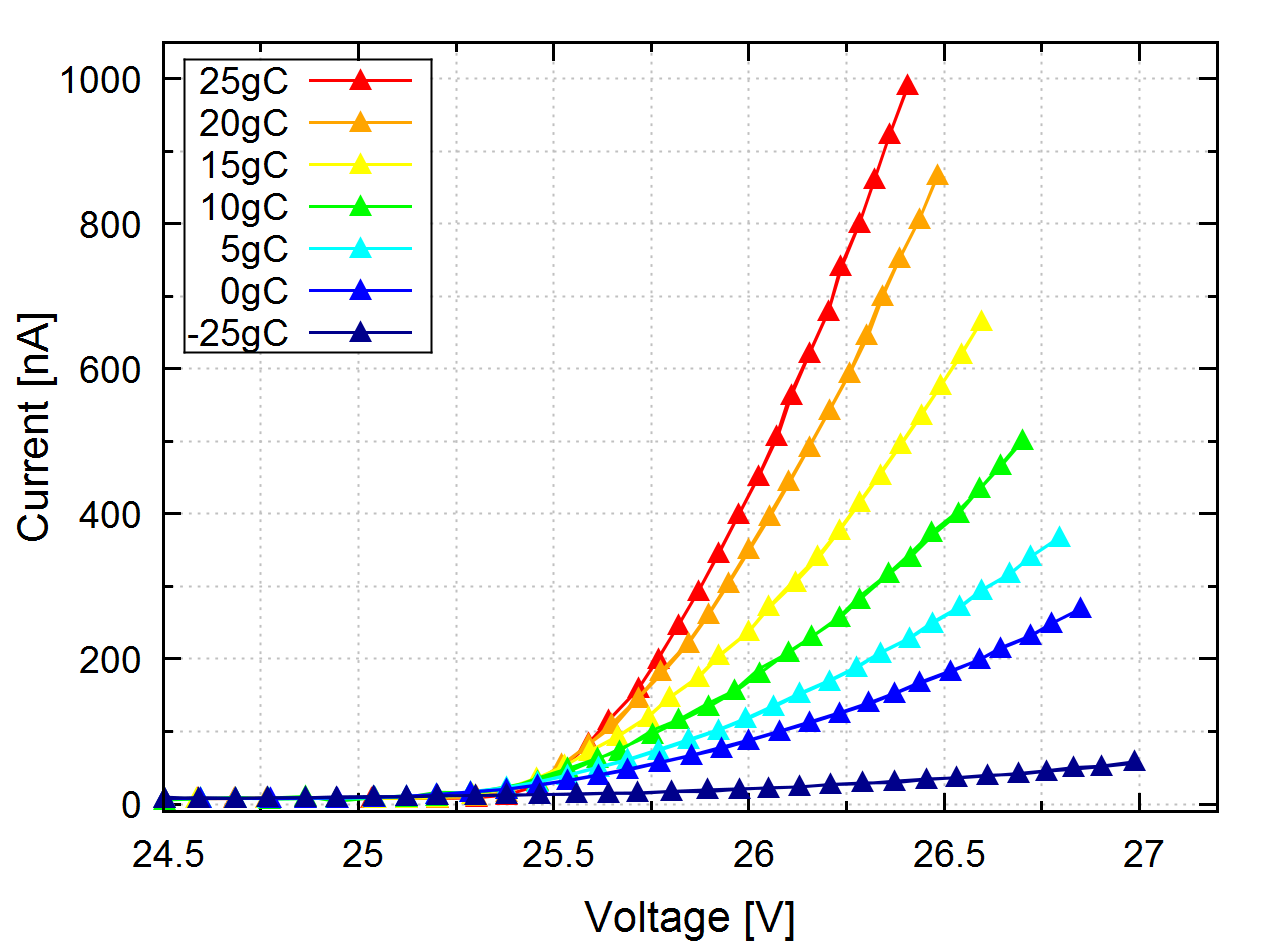
\includegraphics[width=0.49\textwidth]{./plots/iu_curve/4x1n6.png}}
	\hfill
	\subfloat[(h)-configuration logscale] {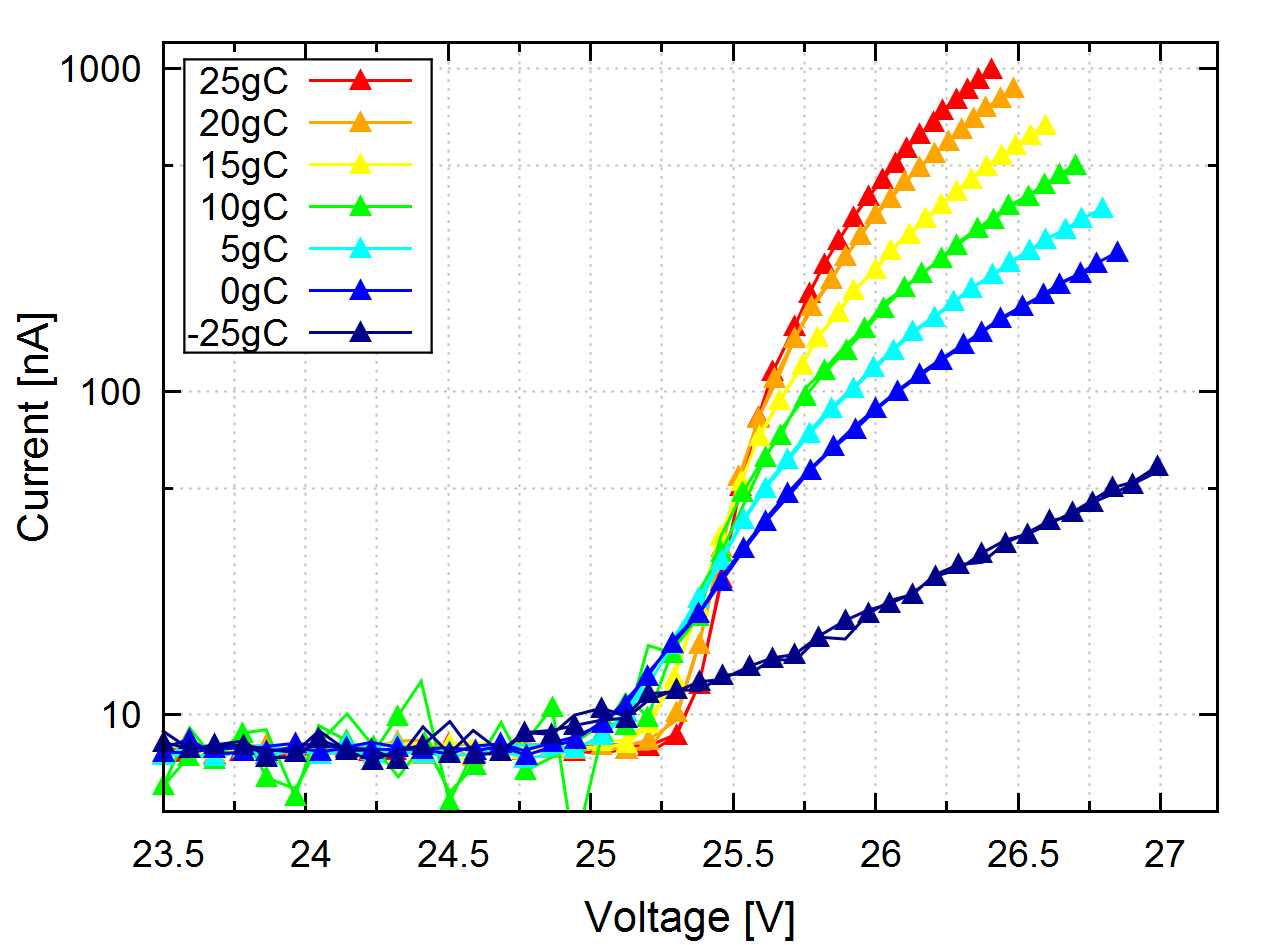
\includegraphics[width=0.49\textwidth]{./plots/iu_curve/4x1n6_log.png}}
	\hfill
	\subfloat[(p)-configuration] {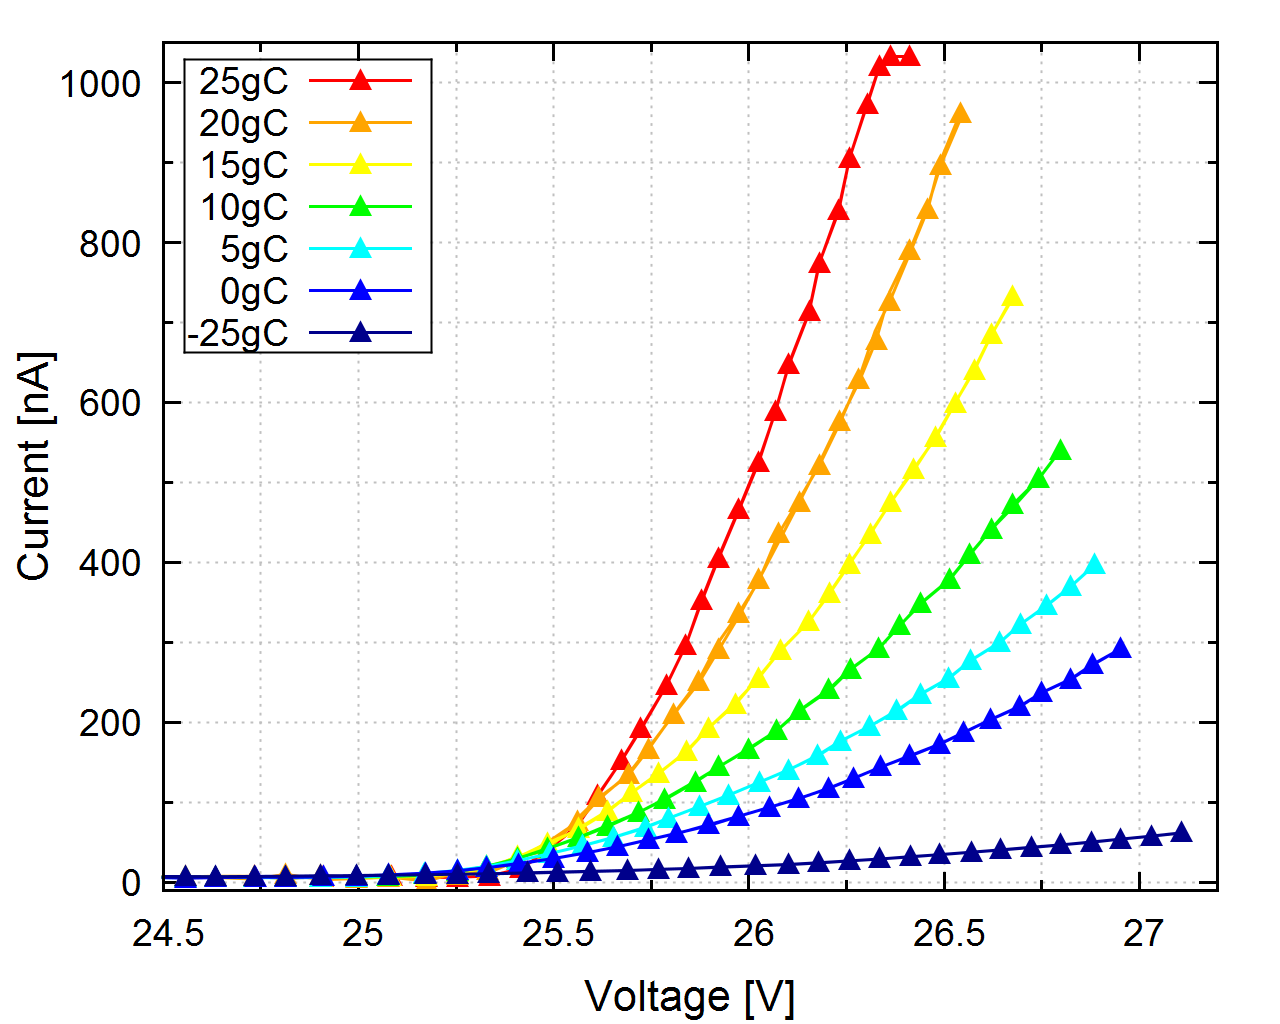
\includegraphics[width=0.49\textwidth]{./plots/iu_curve/4x1n6p.png}}
	\hfill
	\subfloat[(p)-configuration logscale] {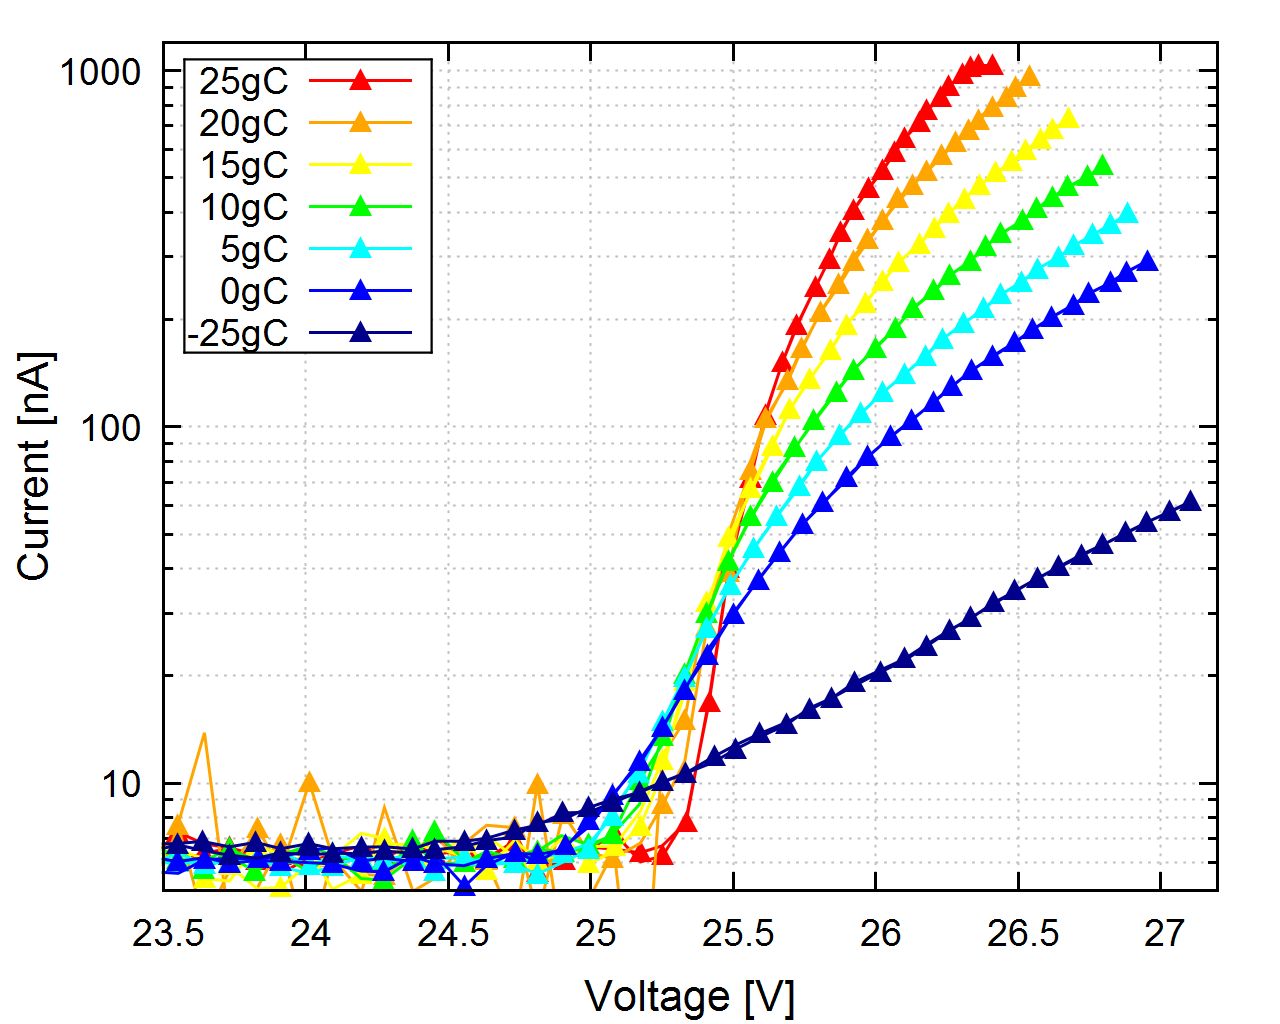
\includegraphics[width=0.49\textwidth]{./plots/iu_curve/4x1n6p_log.png}}
	\hfill
	\caption[IV-curve of different board configurations]{Comparison of different board configurations. For (h)- and (p)-configuration the same SiPMs were used. }
	\label{fig:ch4:IV_comparison}
\end{figure}
The IV-curves were scanned from $I=\SI{0}{\nano\ampere}$ to $I\approx\SI{1000}{\nano\ampere}$ and back to $I=\SI{0}{\nano\ampere}$. The step range is given by the digital potentiometer (10bit) on the HV board, a small hysteresis for the current is known (see \cite{chris}). For each potentiometer position (voltage), the current is measured 100 times and is then averaged. This results in two IV-curves per SiPM which should improve precision. It has to be mentioned that the voltage and current measurements are not fully calibrated yet, so a small offset might occur. This is not considered in this thesis, since qualitative comparison between the boards is sufficient.  \par 
The IV-curves for the different configurations are shown in figure \ref{fig:ch4:IV_comparison}. Plot (a) and (b) show the curves of a single SiPM. The temperature is color coded from warm (red) to cold (dark blue). It can be seen that the current rises exponentially when the breakdown voltage is exceeded. At this point, the local field strength is high enough to create avalanches. This process is temperature dependent: for lower temperatures, the generation of thermal electrons as free charge carriers able to start an avalanche is suppressed. \par 
The temperature also affects the breakdown voltage. A negative breakdown coefficient $k$ (in [$\si{\milli\volt\per\kelvin}$]) occurs in \tit{Zener diodes}: due to high doping, the band structures are heavily curved and show a steep slope. For higher temperatures, an electron can tunnel from the valence to the conduction band more easily. For avalanche diodes a positive $k$ is observed. Lower temperature suppresses electron-phonon scattering which increases the \tit{mean free path} (average distance between collisions) of electrons. This facilitates the development of avalanches and leads to a reduced breakdown voltage.\par 
Compared to a single SiPM, the parallel and hybrid configurations show higher currents. Each SiPM in the array is driven with the same voltage and contributes a net current to the overall current. Hence, the current should be the sum of the net currents. Therefore, breakdown and operation voltage can not be adjusted for each SiPM in an array but has to be treated altogether. This will be discussed later.

\section{Breakdown and operation voltage}


\begin{figure}[t]
	\subfloat[(s)-configuration] {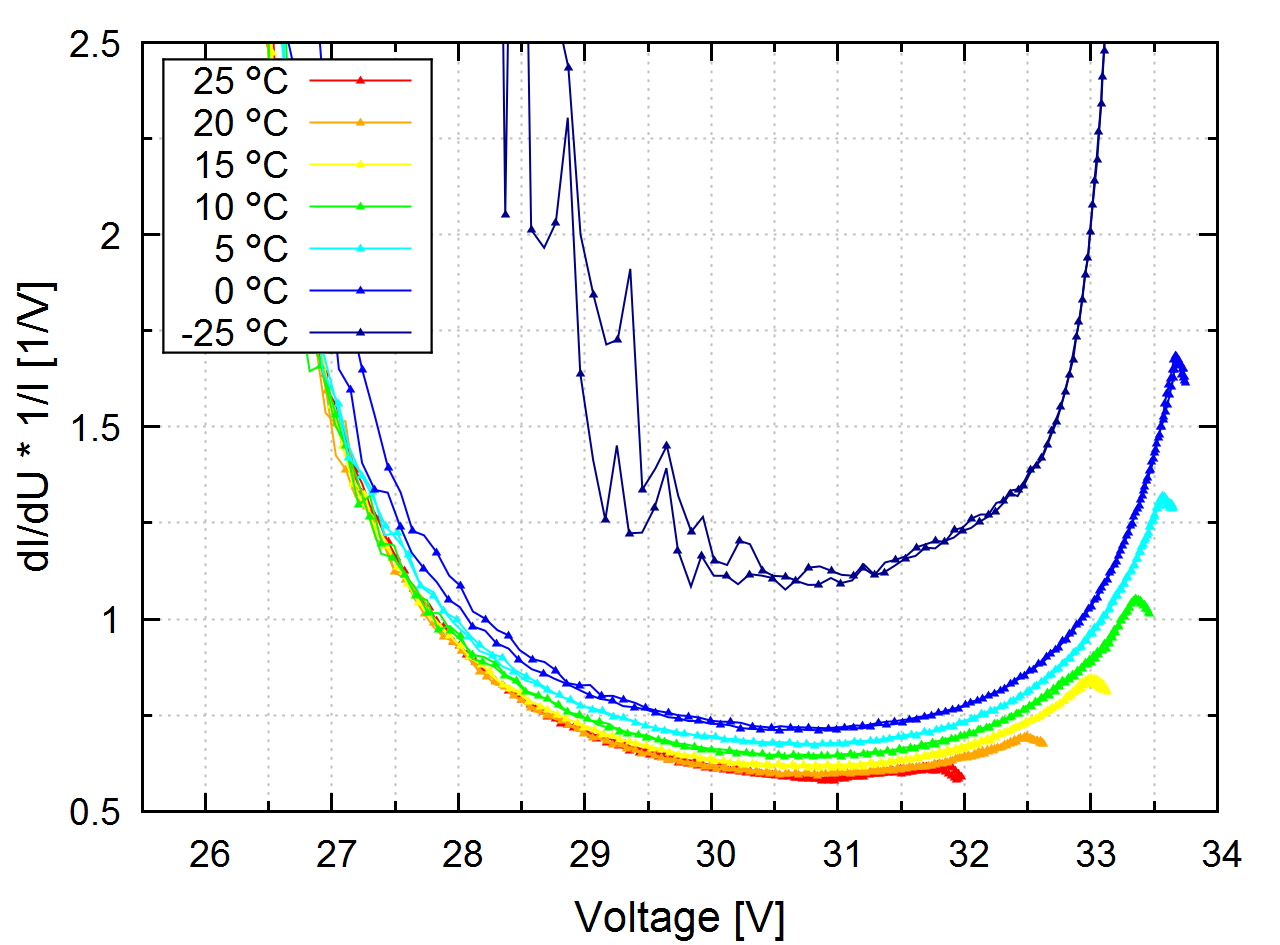
\includegraphics[width=0.49\textwidth]{./plots/iu_curve/1x1n2_op.png}}
	\hfill
	\subfloat[(h)- and (p)-configuration] {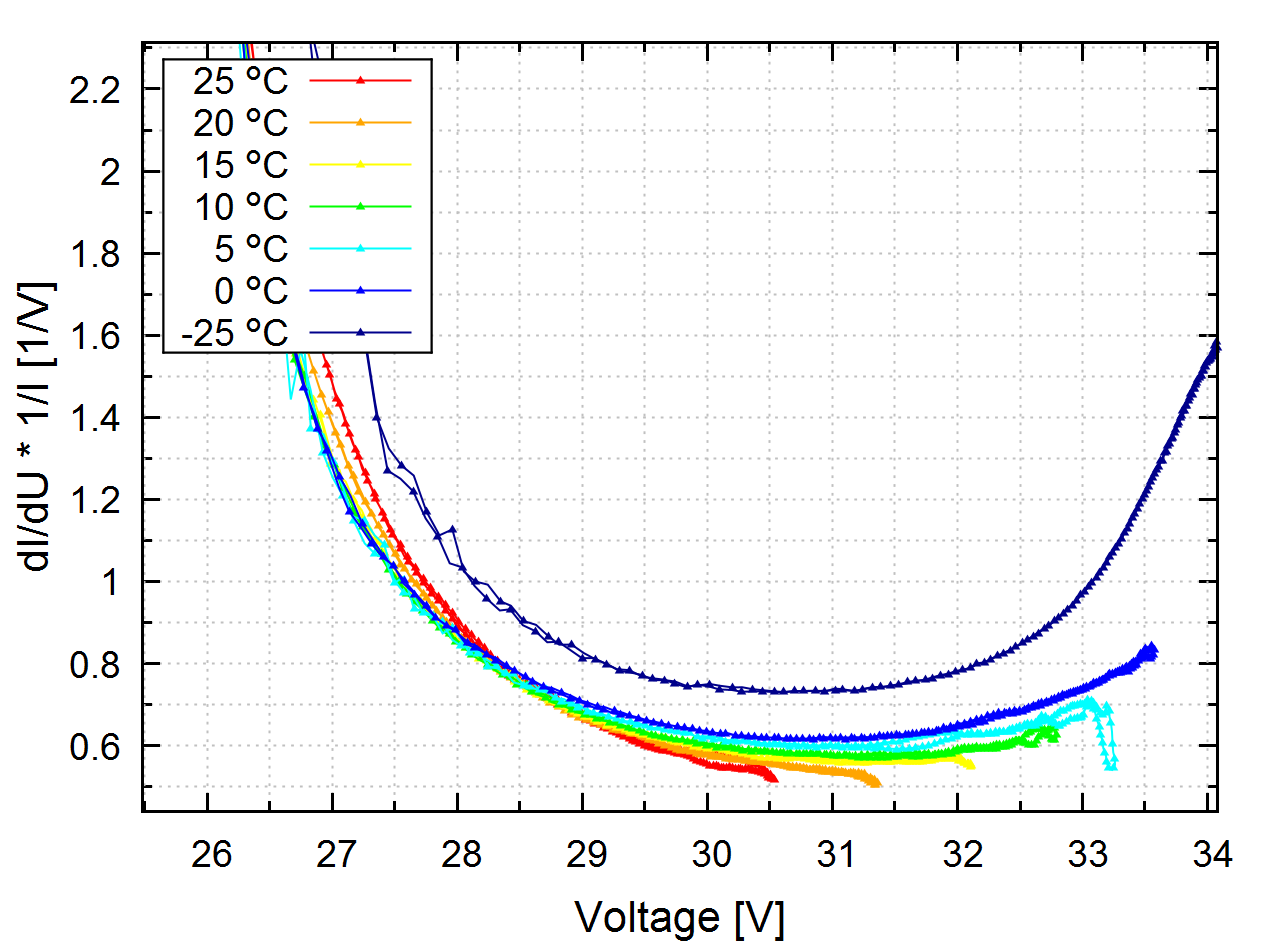
\includegraphics[width=0.49\textwidth]{./plots/iu_curve/4x1n6_op.png}}
	\hfill
	\caption[Comparison of operation voltages]{Comparison of operation voltages. The hybrid and parallel configurations show similar properties.}
	\label{fig:ch4:op_fits}
\end{figure}


The temperature dependence of the breakdown and operation voltages was extracted from the IV-curves. \par 
To calculate the temperature constant $k$, the breakdown voltage was determined. For this, the IV-curves were plotted in logarithmic scale on the y-axis (see \ref{fig:ch4:IV_comparison}). The intersection of a linear fit for the dark current and a second order polynomial fit for the breakdown region provides the sought voltage. The fits can be found in the appendix (see \ref{ap:B:breakdown_fits_single} and \ref{ap:B:breakdown_fits_hybrid}). \par 
\begin{table}[b!]
	\centering
	\begin{tabular}{ c|cc|cc } \toprule[2pt]
		& \multicolumn{2}{c|}{(s)-configuration} & \multicolumn{2}{c}{(h)- and (p)-configuration} \\
		T [$\si{\degreeCelsius}]$ & $V_{OP}$ [$\si{\volt}$] & $V_{BD}$ [$\si{\volt}$] & $V_{OP}$ [$\si{\volt}$] & $V_{BD}$ [$\si{\volt}$]  \\ \midrule
		-25 & $30.78\pm 3.99$ & $24.62\pm 2.89$ & $30.72\pm 0.47$ & $24.40\pm 3.67$ \\
		0 & $30.67\pm 0.42$ & $25.50\pm 0.60$ & $30.89\pm 0.15$ & $24.78\pm 0.03$ \\
		5 & $30.72\pm 0.32$ & $24.93\pm 0.15$ & $31.01\pm 0.59$ & $24.87\pm 0.04$ \\
		10 & $30.70\pm 0.35$ & $25.11\pm 0.44$ & $31.20\pm 0.32$ & $25.04\pm 0.04$ \\
		15 & $30.74\pm 0.28$ & $25.30\pm 0.14$ & $31.32\pm 0.68$ & $25.08\pm 0.01$ \\
		20 & $30.80\pm 0.23$ & $25.35\pm 0.05$ & $31.57\pm 0.75$ & $25.18\pm 0.03$ \\
		25 & $30.87\pm 0.45$ & $25.51\pm 0.23$ & $31.04\pm 2.11$ & $25.20\pm 0.06$ \\
		\midrule
		 & $k_{OP}$ [$\si{\milli\volt\per\kelvin}$] & $k_{BD}$ [$\si{\milli\volt\per\kelvin}$] & $k_{OP}$ [$\si{\milli\volt\per\kelvin}$] & $k_{BD}$ [$\si{\milli\volt\per\kelvin}$]  \\
		 & $6.79\pm 1.34$ & $23.66\pm 5.10$ & $23.67\pm 2.90$ & $19.30\pm 1.51$ \\
		\bottomrule[2pt]
	\end{tabular}
	\caption[Fit results for operation and breakdown voltages]{Fit results for operation and breakdown voltages. Since the same SiPMs were used for (h)- and (p)-configuration the results are the similar.}
	\label{ch4:tab:IV_cata}
\end{table}    
Finding the optimal operation voltage $V_{OP}$ is important for maintaining the detector in the experiment with good a signal-to-noise ratio. One has to trade off high gain and low noise to get sufficient amplification without amplifying too much noise. In order to find this working point, the derivative\footnote{The method for deriving the data is described in \ref{ap:B:sec:derivation}} of the IV-curve has been divided by the current $I(V)$ which results in a local minimum some volts beyond breakdown. The minimum of this relative slope $\dv{I}{V}\frac{1}{I(V)}$ is the voltage where the effect of altering the voltage has the smallest effect in the region beyond breakdown, so small voltage changes should not be as problematic as at other positions. Furthermore, for higher voltages the noise is disproportionately amplified due to high current compared to the amplification of the signal. The minimum was determined by fitting the region with a second order polynomial, again the fits can be found in the appendix (figures \ref{ap:B:optimal_fits_single} and \ref{ap:B:optimal_fits_hybrid}). \par
The results are listed in table \ref{ch4:tab:IV_cata}. The temperature dependence can clearly be seen, the coefficients are positive and and coincide with data provided by KETEK (see data sheet \cite{ketek}). The linear fits are shown in figure \ref{fig:ch4:breakdown_fits}. The (s)-configuration as a single SiPM has a slightly higher $k_{BD}$ with a large error due to difficulties in fitting the $\SI{-25}{\degreeCelsius}$ data (low current).  The operation voltage is roughly $V_{OP}=V_{BD}+\SI{5}{\volt}$ and rises slowly with higher temperature, whereas multiple SiPMs show a steeper slope due to higher intrinsic noise. This suggests to operate the SiPM-boards at $30-31\si{\volt}$ when no precise source is available. Again, the voltage measurement is not calibrated yet, so this is just a rough recommendation. 

 

\begin{figure}[t]
	\subfloat[(s)-configuration] {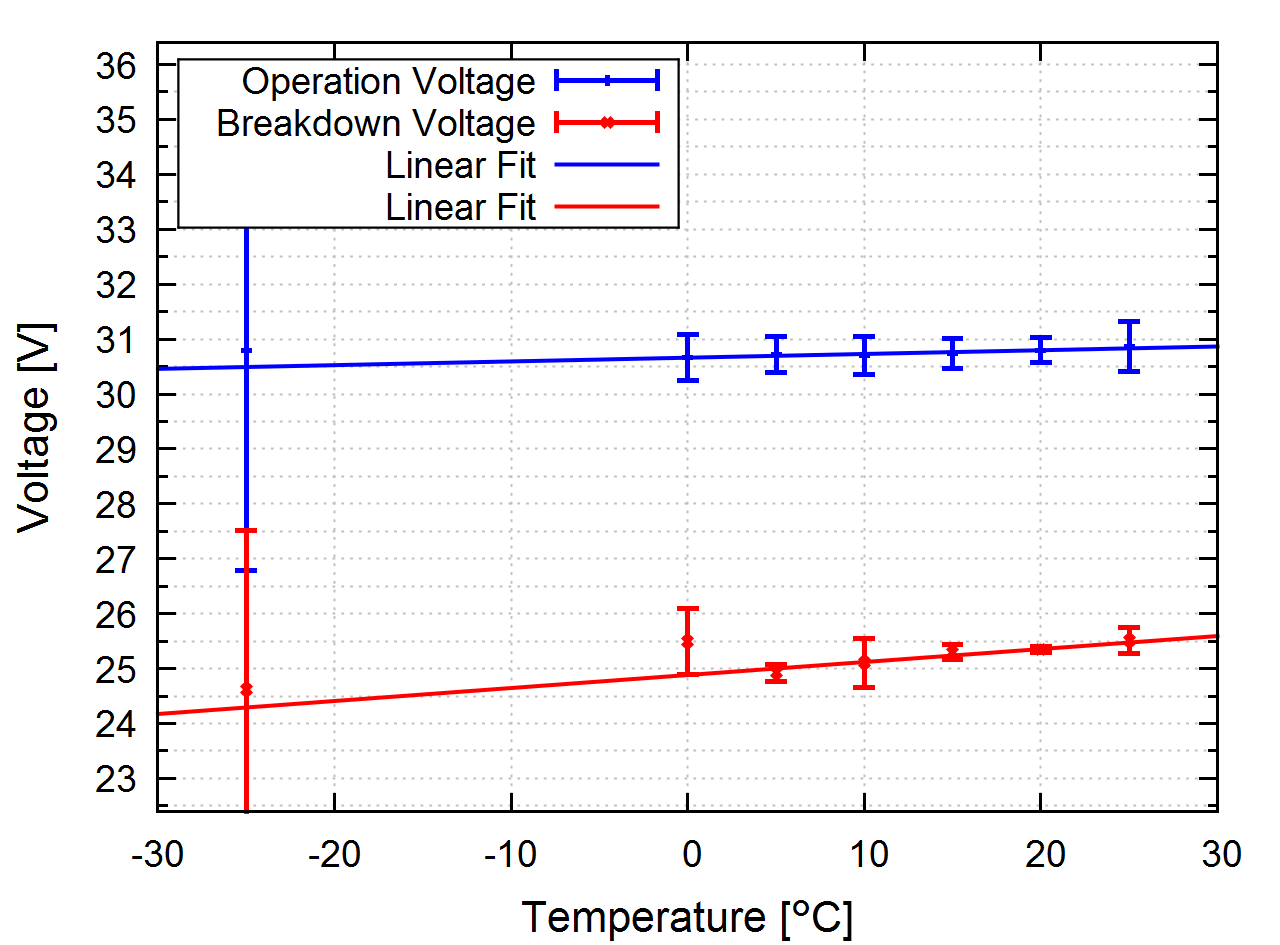
\includegraphics[width=0.49\textwidth]{./plots/iu_curve/1x1n2_fits.png}}
	\hfill
	\subfloat[(h)- and (p)-configuration] {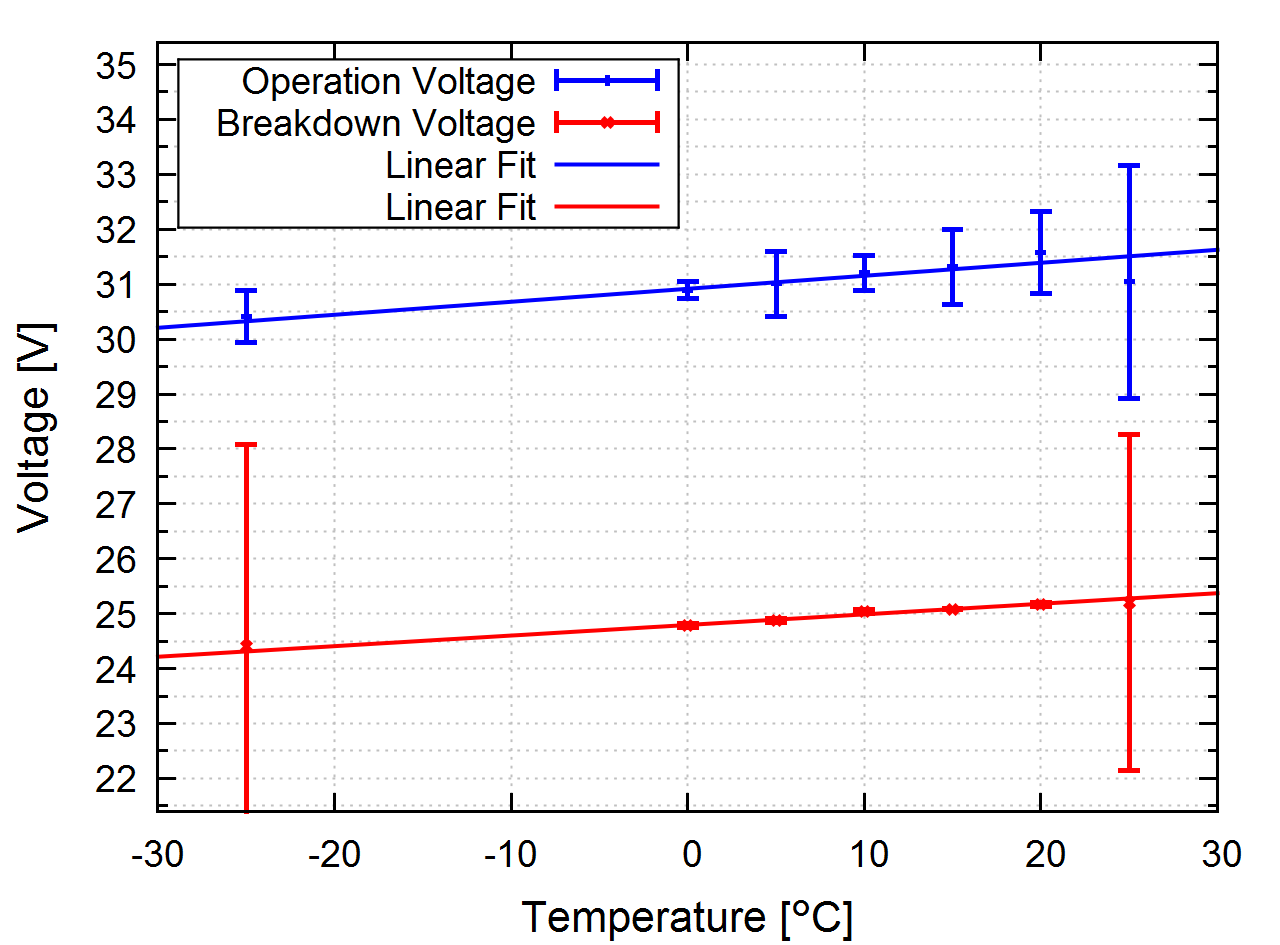
\includegraphics[width=0.49\textwidth]{./plots/iu_curve/4x1n6_fits.png}}
	\hfill
	\caption[Comparison of breakdown and operation voltages]{Comparison of breakdown and operation voltages. The hybrid and parallel configurations show similar properties. Note the positive slope.}
	\label{fig:ch4:breakdown_fits}
\end{figure}


\section{Dark count rate}

Measuring the dark count rate and visualizing the ``dark spectrum" is important for determining a proper threshold level in further experiments when it comes to processing signals right above the noise. \par 
Dark signals are thermally generated signals by electrons with sufficient energy to generate an avalanche. Since the built-in-potential is high, even small thermal energies cause electrons to create avalanches. This results in a high count rate of dark events. \par 
Due to the unique design of the SiPM with discrete micro cell signals, single firing cells contribute most to the count rate. Multiple coincident dark events result in a higher signal whereas the rate for these events is much lower. The probability for a higher number of coincident dark events is close to zero, so the threshold can be set to a level right above a certain number of cells. \par 
\begin{figure}[t]
	\subfloat[(s)-configuration. $\SI{5}{\nano\second}$/div and $\SI{20}{\milli\volt}$/div. Threshold at $\SI{-12}{\milli\volt}$.] {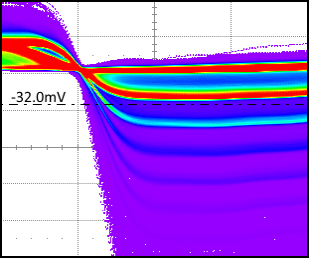
\includegraphics[width=0.475\textwidth]{./plots/darc_electron_spectrum/test16.png}}
	\hfill
	\subfloat[(h)-configuration. $\SI{5}{\nano\second}$/div and $\SI{5}{\milli\volt}$/div. Threshold at $\SI{-8}{\milli\volt}$.] {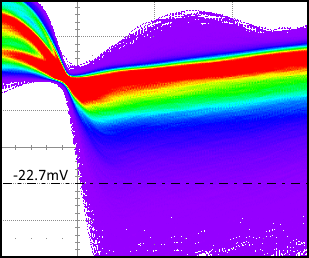
\includegraphics[width=0.475\textwidth]{./plots/darc_electron_spectrum/spectrum_hybrid.png}}
	\hfill
	\caption[Dark spectrum of single and multiple SiPM-configurations]{Dark spectrum of (s)- and (h)-configuration. The single SiPMs shows distinct peaks whereas multiple SiPMs exhibit a more blurred spectrum.}
	\label{fig:ch4:darc_spectrum}
\end{figure}
\begin{figure}[b!]
	\floatbox[{\capbeside\thisfloatsetup{capbesideposition={left,center},capbesidewidth=6cm}}]{figure}[\FBwidth]
	{\caption[Pulse hight spectrum]{Pulse hight spectrum for dark events with single and multiple SiPMs in logarithmic scale and normalized counts per millivolt. The single SiPM shows distinct peaks whereas the spectrum of the hybrid configuration is more blurred and the peaks can only be estimated. }    
		\label{fig:ch4:pulse_hight_hist}}
	{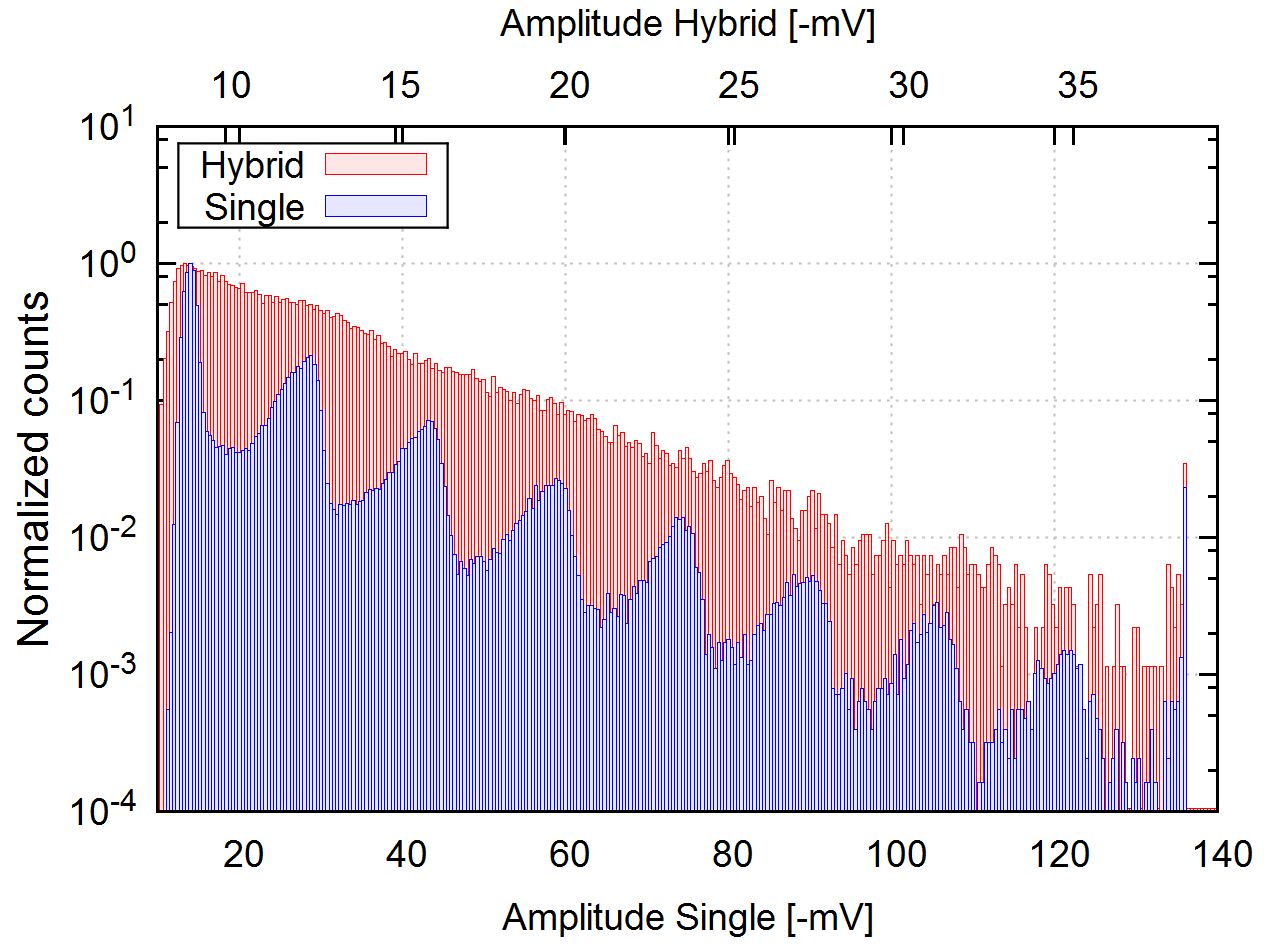
\includegraphics[width=0.6\textwidth]{./plots/darc_electron_spectrum/Counts_multi.png}}
\end{figure}
To get a first qualitative scrutiny of the dark spectrum, a single SiPM and a hybrid board were wrapped light tight with black tape and then stored in a closed aluminum box. The signals were then amplified by a preamplifier in order to get a better resolution of the spectrum. The preamp was operated with $\SI{5}{\volt}$, the SiPM-board with $\SI{30}{\volt}$. The raw signal was tracked and monitored by a \tit{LeCroy Waverunner 104MXi-A 1GHz} oscilloscope. \par 
With persistence setup, a waveform-picture of more than 10.000 signals was taken for both configurations which can be seen in figure \ref{fig:ch4:darc_spectrum}. The single SiPM shows distinct peaks, the discrete signal height for a single cell can be roughly estimated as \SI{15}{\milli\volt}. The spectrum of multiple SiPMs is more blurred due to slightly different characteristics of each SiPM in the array. Still, a stepwise distribution of signals can be observed which also can be used to estimate the number of firing cells. \par  
This can be represented distinctly by plotting the pulse height. The histogram \ref{fig:ch4:pulse_hight_hist} visualizes the counts per millivolt in logarithmic scale and normalized count rate per millivolt. The single SiPM shows distinct peaks with a gap of roughly \SI{15}{\milli\volt}, the spectrum of multiple SiPMs is blurred and the steps are not as distinct as for a single SiPM. \par 
\begin{figure}[t]
	\centering
	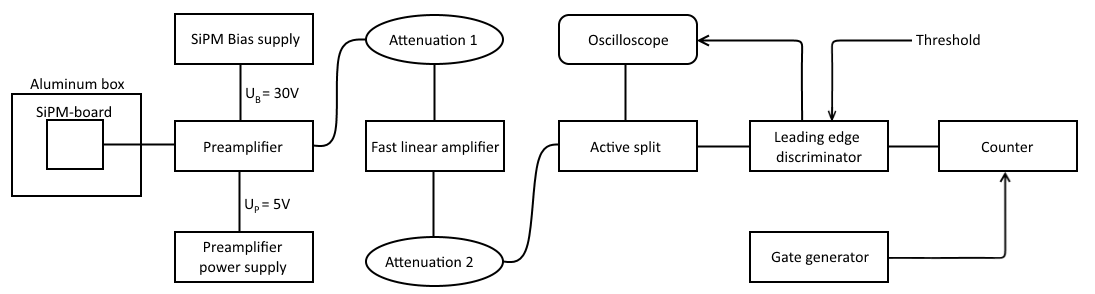
\includegraphics[width=1\linewidth]{./graphics/ch4/scheme_count_rate.png}
	\caption[Schematic of the dark count rate measurement]{Schematic of the dark count rate measurement.}
	\label{fig:ch4:scheme_rate}
\end{figure}
\begin{figure}[b]
	\floatbox[{\capbeside\thisfloatsetup{capbesideposition={right,center},capbesidewidth=0.4\linewidth}}]{figure}[\FBwidth]
	{\caption[Slope of the dark count rate]{Normalized slope of dark count rate. The single SiPM (blue) shows distinct steps whereas the other configurations do not show such a behavior.}    
		\label{fig:ch4:slope_countrate}}
	{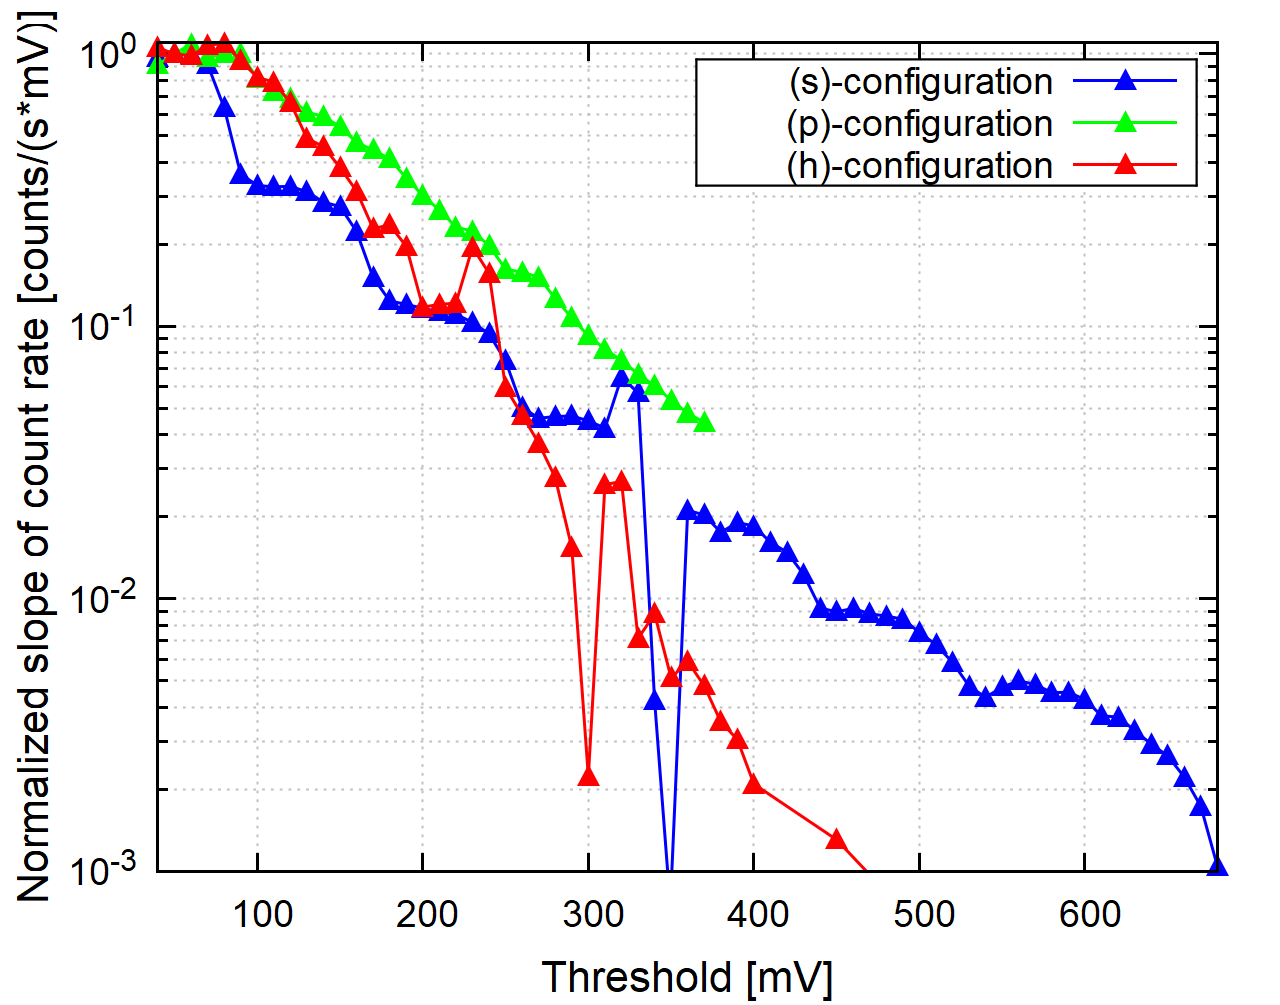
\includegraphics[width=0.6\textwidth]{./plots/darc_electron_spectrum/slope_countrate.png}}
\end{figure}
To measure the count rate of the different configurations, the setup shown in figure \ref{fig:ch4:scheme_rate} was used. Again, the SiPM-boards were wrapped light tight, stored in the aluminum box and operated by the preamplifier. To exploit the whole range of the available leading edge discriminator (Lecroy 623B, threshold $\SI{-30}{\milli\volt}$ to $\SI{-800}{\milli\volt}$), some further amplifications had to be made. A fast linear amplifier (FTA810L from GSI, V=800, $\tau\leq\SI{10}{\nano\second}$) was used for this reason, but to avoid saturation of this amplifier and to further fine tune the signal range, passive attenuators were utilized before and after the amplifier. An active split divided the signal for monitoring the threshold level of the discriminator. A megahertz counter (from Uni Bonn) was gated by a gate generator (Lecroy 222) to count the signals for $\SI{10}{\second}$. \par 
The first derivative was calculated\footnote{Again, the method used is described in \ref{ap:B:sec:derivation}} from the retrieved data to emphasize the expected drop in count rate. Figure \ref{fig:ch4:slope_countrate} shows this normalized slope of count rate in logarithmic scale. The single SiPM (blue) yields the unique stepwise drop in count rate with a width of approximately $\SI{80}{\milli\volt}$ per step. Again, the array configurations do not show such a distinct behavior. \par 
The absolute count rate and slope of each setup for prominent threshold levels is given in table \ref{ch4:tab:count_rate}, note that the edges of the first five steps of the single SiPM are used for highlighting the discrete spectrum. This behavior could not be found in the array setups, the slope is nearly linear which indicates a exponential decrease in count rate. \par 

\begin{table}[t]
	\centering
	\begin{tabular}{ c|cc|cc|cc } \toprule[2pt]
		& \multicolumn{2}{c|}{(s)-configuration} & \multicolumn{2}{c|}{(h)-configuration} & \multicolumn{2}{c}{(p)-configuration} \\
		TH [$\si{\milli\volt}]$ & $f$ [$\si{\kilo\hertz}$] & Slope [$\si{\kilo\hertz\per\volt}$] & $f$ [$\si{\kilo\hertz}$] & Slope [$\si{\kilo\hertz\per\volt}$] & $f$ [$\si{\kilo\hertz}$] & Slope [$\si{\kilo\hertz\per\volt}$] \\ \midrule
		-30 & 1827 & 190 & 4089 & 360 & 3389 & 300 \\
		-80 & 866 & 180 & 2335 & 400 & 2274 & 200 \\ \midrule
		-90 & 786 & 60 & 2006 & 330 & 2024 & 225 \\
		-160 & 355 & 60 & 603 & 110 & 963 & 110 \\ \midrule
		-170 & 319 & 20 & 508 & 100 & 859 & 100 \\
		-250 & 141 & 19 & 87.6 & 23 & 340 & 40 \\ \midrule
		-260 & 121 & 10 & 70.9 & 17 & 304 & 35 \\
		-340 & 50.9 & 9.0 & 13.7 & 5.0 & 119 & 14 \\ \midrule
		-350 & 48.9 & 2.9 & 12.4 & 1.3 & 107 & 12.5 \\
		-430 & 27.6 & 3.0 & 1.77 & 0.2 & $-$ & $-$ \\ \midrule
		-440 & 25.6 & 1.9 & $-$ & $-$ &  $-$ &  $-$ \\
		-500 & 15.1 & 1.6 & $-$ &  $-$ &  $-$ &  $-$ \\
		-600 & 4.8 & 0.7 & $-$ & $-$ &  $-$ &  $-$ \\
		-720 & 0 & 0 & $-$ & $-$ &  $-$ &  $-$ \\
		\bottomrule[2pt]
	\end{tabular}
	\caption[Absolute dark count rate]{Absolute dark count rate for different configurations. The steps (drop in count rate) for the single SiPM are highlighted by horizontal lines.}
	\label{ch4:tab:count_rate}
\end{table}  

For the single SiPM, the rate has been measured until no counts were registered within $\SI{10}{\second}$. This point is reached at $\SI{-720}{\milli\volt}$. The data indicates steps with a width of $\SI{80}{\milli\volt}$, so the upper limit for coincident firing cells is nine cells at the same time. The rate for single cells lies in the megahertz region, for five cells in the low kilohertz region, for seven cells some hundreds of hertz. The rate for the array setups is nearly four times the rate of a single cell. \par 
Further work on comparing pulse signals, timing response and energy measurements will be shown in chapter \ref{ch:timing}, in which the different configurations were mounted to a plastic scintillator of type \tit{EJ-248M} from \tit{ELJEN} and inorganic crystals, LYSO and \pwo{}.









